\section{Flex-I (model ID: 26)}
The Flex-I model (fig.~\ref{fig:26_schematic}) is the part of a model development exercise \citep{Fenicia2008}. It has 4 stores and 10 parameters ($I_{max}$, $UR_{max}$, $\beta$, $D$, $Perc_{max}$, $L_p$, $N_{lag,f}$, $N_{lag,s}$, $K_f$ and $K_s$). The model aims to represent:

\begin{itemizecompact}
\item Interception by vegetation;
\item Infiltration and saturation excess flow based on a distribution of different soil depths;
\item A split between fast saturation excess flow and preferential recharge to a slow store;
\item Percolation from the unsaturated zone to a slow runoff store.
\end{itemizecompact}

\subsection{MARRMoT model name}
m\_26\_flexi\_10p\_4s \\

% Equations
\subsection{Model equations}

% Model layout figure
{ 																	% This ensures it doesn't warp text further down
\begin{wrapfigure}{l}{7cm}
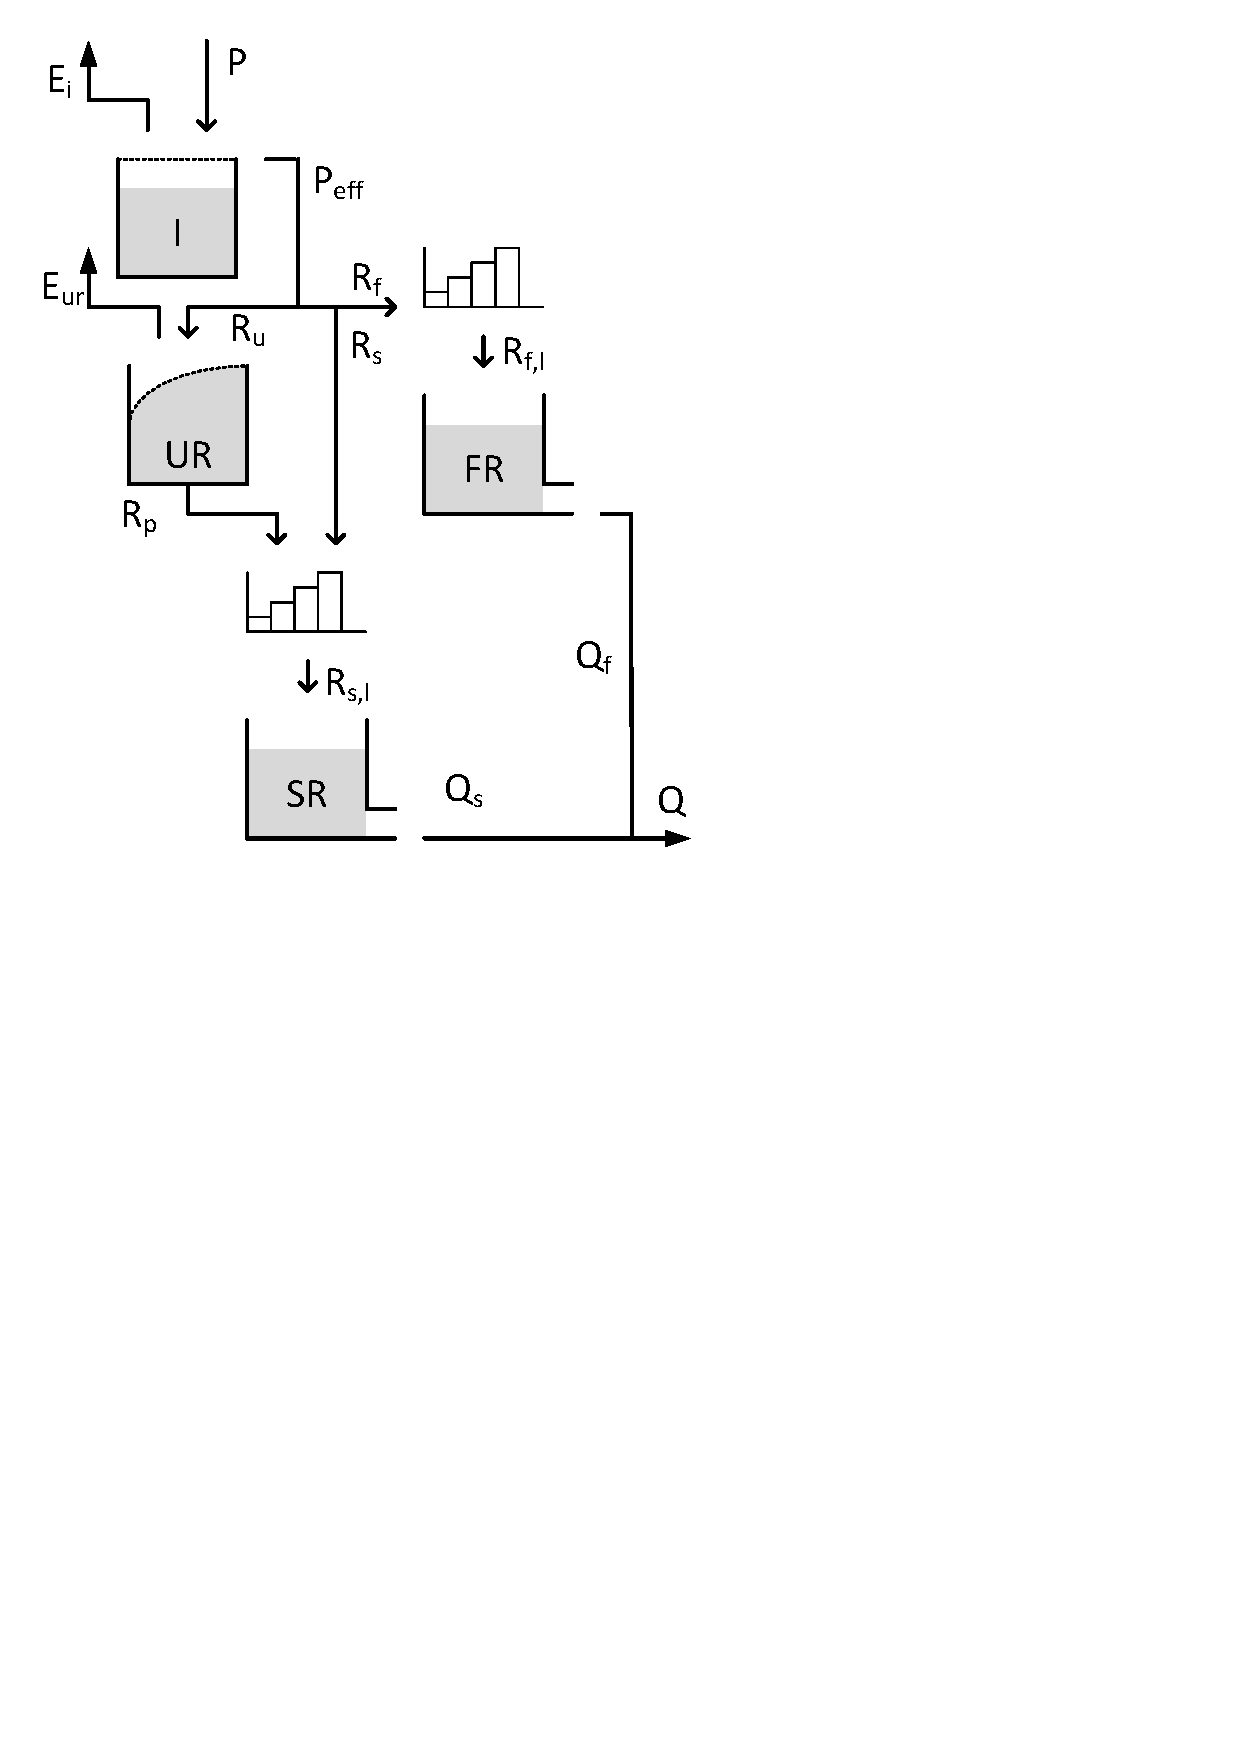
\includegraphics[trim=1cm 15cm 7cm 1cm,width=7cm,keepaspectratio]{./AppA_files/26_schematic.pdf}
\caption{Structure of the Flex-I model} \label{fig:26_schematic}
\end{wrapfigure}

\begin{align}
	\frac{dI}{dt} &= P-E_i-P_{eff} \\
	E_i &= \begin{cases}
		Ep &\text{, if } I > 0\\
		0 &\text{, otherwise }\\
	\end{cases}\\
	P_eff &= \begin{cases}
		P &\text{, if } I \geq I_{max}\\
		0 &\text{, otherwise }\\
	\end{cases}	
\end{align}

Where I is the current interception storage [mm], P $[mm/d]$ incoming precipitation, $E_i$ $[mm/d]$ evaporation from the interception store and $P_{eff}$  $[mm/d]$ interception excess routed to soil moisture. Evaporation occurs at the potential rate $E_p$ [mm/d] whenever possible. Interception excess occurs when the interception store exceeds its maximum capacity $I_{max}$ [mm].

} % end of wrapfigure fix
\vspace{1cm}

\begin{align}
	\frac{dUR}{dt} &= R_u - E_{ur} - R_p \\
	R_U &= (1 - C_r) * P_{eff}\\
	C_r &= \Big[1+exp\Big(\frac{-UR/UR_{max} + 1/2}{\beta}\Big)\Big]^{-1}\\
	%R_u &= (1 - \Big[1+exp\Big(\frac{-UR/UR_{max} + 1/2}{\beta}\Big)\Big]^{-1}) * P_{eff}\\
	E_{ur} &= E_p * min\Big(1, \frac{UR}{UR_{max}} \frac{1}{L_p}\Big)\\
	P_s&= Perc_{max} * \frac{-UR}{UR_{max}}
\end{align}
  
Where UR is the current storage in the unsaturated zone [mm]. $R_u$ $[mm/d]$ is the inflow into UR based on its current storage compared to maximum storage $UR_{max}$ [mm] and a shape distribution parameter $\beta$ [-].  $E_{ur}$ the evaporation $[mm/d]$ from UR which follows a linear relation between current and maximum storage until a threshold $L_p$ [-] is exceeded. $P_s$ is the percolation from UR to the slow reservoir SR $[mm/d]$, based on a maximum percolation rate $Perc_{max}$ [mm], relative to the fraction of current storage and maximum storage. $P_{eff}$ is routed towards the unsaturated zone based on $Cr$, with the remainder being divided into preferential recharge $R_s$ $[mm/d]$ and fast runoff $R_f$ $[mm/d]$:

\begin{align}
	R_s &= (P_{eff} - R_u)*D\\
	R_f &= (P_{eff} - R_u)*(1-D)
\end{align}

Where $R_s$ and $R_f$ are the flows $[mm/d]$ to the slow and fast runoff reservoir respectively, based on runoff partitioning coefficient D [-]. Both are lagged by linearly increasing triangular transformation functions with parameters $N_{lag,s}$ [d] and $N_{lag,f}$ [d] respectively, that give the number of days over which $R_s$ and $R_f$ need to be transformed. Percolation $R_p$ is added to $R_s$ before the transformation to $R_{s,l}$ occurs.

\begin{align}
	\frac{dFR}{dt} &= R_{f,l} - Q_f\\
	Q_f &= K_f * FR 
\end{align}

Where FR is the current storage [mm] in the fast flow reservoir. Outflow $Q_f$ $[mm/d]$ from the reservoir has a linear relation with storage through time scale parameter $K_f$ [$d^{-1}$]. 

\begin{align}
	\frac{dSR}{dt} &= R_{s,l} - Q_s \\
	Q_s &= K_s * SR 
\end{align}

Where SR is the current storage [mm] in the slow flow reservoir. Outflow $Q_s$ $[mm/d]$ from the reservoir has a linear relation with storage through time scale parameter $K_s$ [$d^{-1}$]. Total outflow Q  $[mm/d]$:

\begin{equation}
	Q = Q_f + Q_s
\end{equation}

\subsection{Parameter overview}
% Table generated by Excel2LaTeX from sheet 'Sheet1'
\begin{table}[htbp]
  \centering
    \begin{tabular}{lll}
    \toprule
    Parameter & Unit  & Description \\
    \midrule
    $I_{max}$ & $mm$  & Maximum interception storage \\
    $UR_{max}$ & $mm$  & Maximum soil moisture storage \\
    $\beta$ & $-$   & Shape parameter \\
    $D$   & $-$   & Fraction effective precipitation to slow store \\
    $Perc_{max}$ & $mm~d^{-1}$ & Maximum percolation rate \\
    $L_p$ & $-$   & Wilting point as fraction of $UR_{max}$ \\
    $N_{lag,f}$ & $d$   & Unit Hydrograph time base \\
    $N_{lag,s}$ & $d$   & Unit Hydrograph time base \\
    $K_f$ & $d^{-1}$ & Runoff coefficient \\
    $K_s$ & $d^{-1}$ & Runoff coefficient \\
    \bottomrule
    \end{tabular}%
  \label{tab:addlabel}%
\end{table}%
